\chapter{Consultes d'arbres}

\index{consulta d'arbre}

En aquest capítol es tracta de tècniques per processar consultes sobre
subarbres i camins d'un arbre arrelat, com ara les següents:

\begin{itemize}
\item quin és el $k$-èssim avantpassat d'un node?
\item quina és la suma dels valors del subarbre d'un node?
\item quina és la suma dels valors en un camí entre dos nodes?
\item quin és l'avantpassat comú més baix a dos nodes?
\end{itemize}

\section{Trobar avantpassats}

\index{avantpassat}

El $k$-èssim \key{avantpassat} d'un node $x$ en un arbre arrelat és el
node al qual arribarem si ens movem $k$ nivells amunt d'un node
$x$. Sigui $\texttt{ancestor}(x,k)$ el $k$-èssim avantpassat d'un node
$x$ (o $0$ si no existeix). Per exemple, a l'arbre següent,
$\texttt{ancestor}(2,1)=1$ i $\texttt{ancestor}(8,2)=4$.
\begin{center}
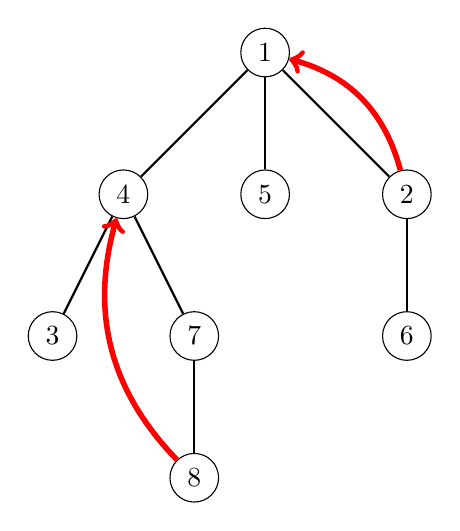
\begin{tikzpicture}[scale=0.9]
\node[draw, circle] (1) at (0,3) {$1$};
\node[draw, circle] (2) at (2,1) {$2$};
\node[draw, circle] (3) at (-2,1) {$4$};
\node[draw, circle] (4) at (0,1) {$5$};
\node[draw, circle] (5) at (2,-1) {$6$};
\node[draw, circle] (6) at (-3,-1) {$3$};
\node[draw, circle] (7) at (-1,-1) {$7$};
\node[draw, circle] (8) at (-1,-3) {$8$};
\path[draw,thick,-] (1) -- (2);
\path[draw,thick,-] (1) -- (3);
\path[draw,thick,-] (1) -- (4);
\path[draw,thick,-] (2) -- (5);
\path[draw,thick,-] (3) -- (6);
\path[draw,thick,-] (3) -- (7);
\path[draw,thick,-] (7) -- (8);

\path[draw=red,thick,->,line width=2pt] (8) edge [bend left] (3);
\path[draw=red,thick,->,line width=2pt] (2) edge [bend right] (1);
\end{tikzpicture}
\end{center}


Una manera fàcil de calcular $\texttt{ancestor}(x,k)$ és fer una
seqüència de $k$ moviments a l'arbre. Tanmateix, la complexitat
temporal d'aquest mètode és $O(k)$, i això pot ser molt lent, perquè
un arbre de $n$ nodes pot tenir una cadena de $n$ descendents.

Afortunadament, amb una tècnica semblant a la del capítol
capítol~\ref{camins-de-successio}, qualsevol valor de
$\texttt{ancestor}(x,k)$ pot calcular-se eficientment en temps $O(\log
k)$ un cop acabat el preprocessament. La idea és precalcular tots els
valors $\texttt{ancestor}(x,k)$ on $k \le n$ és una potència de
dos. Per exemple, els valors de l'arbre anterior són els següents:


\begin{center}
\begin{tabular}{r|rrrrrrrrr}
$x$ & 1 & 2 & 3 & 4 & 5 & 6 & 7 & 8 \\
\hline
$\texttt{ancestor}(x,1)$ & 0 & 1 & 4 & 1 & 1 & 2 & 4 & 7 \\
$\texttt{ancestor}(x,2)$ & 0 & 0 & 1 & 0 & 0 & 1 & 1 & 4 \\
$\texttt{ancestor}(x,4)$ & 0 & 0 & 0 & 0 & 0 & 0 & 0 & 0 \\
$\cdots$ \\
\end{tabular}
\end{center}


El preprocessament triga temps $O(n \log n)$, perquè es calculen
$O(\log n)$ per cada node. Després d'això, qualsevol valor de
$\texttt{ancestor}(x,k)$ es pot calcular en temps $O(\log k)$
representant $k$ com a suma de potències de dos.

\section{Subarbres i camins}

\index{vector recorregut d'arbre}

Un \key{vector recorregut d'arbre} () conté els nodes d'un arbre
arrelat en l'ordre en què una cerca en profunditat des del node arrel
els visitaria. Per exemple, a l'arbre
\begin{center}
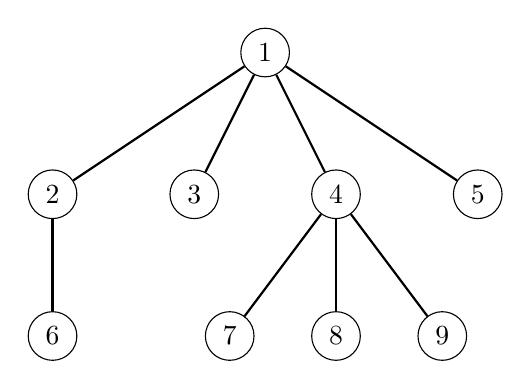
\begin{tikzpicture}[scale=0.9]
\node[draw, circle] (1) at (0,3) {$1$};
\node[draw, circle] (2) at (-3,1) {$2$};
\node[draw, circle] (3) at (-1,1) {$3$};
\node[draw, circle] (4) at (1,1) {$4$};
\node[draw, circle] (5) at (3,1) {$5$};
\node[draw, circle] (6) at (-3,-1) {$6$};
\node[draw, circle] (7) at (-0.5,-1) {$7$};
\node[draw, circle] (8) at (1,-1) {$8$};
\node[draw, circle] (9) at (2.5,-1) {$9$};

\path[draw,thick,-] (1) -- (2);
\path[draw,thick,-] (1) -- (3);
\path[draw,thick,-] (1) -- (4);
\path[draw,thick,-] (1) -- (5);
\path[draw,thick,-] (2) -- (6);
\path[draw,thick,-] (4) -- (7);
\path[draw,thick,-] (4) -- (8);
\path[draw,thick,-] (4) -- (9);
\end{tikzpicture}
\end{center}
una cerca en profunditat es fa com segueix:
\begin{center}
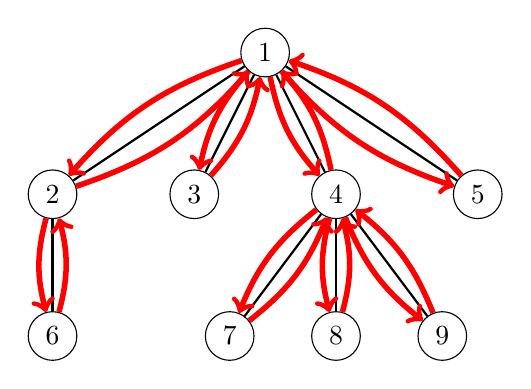
\begin{tikzpicture}[scale=0.9]
\node[draw, circle] (1) at (0,3) {$1$};
\node[draw, circle] (2) at (-3,1) {$2$};
\node[draw, circle] (3) at (-1,1) {$3$};
\node[draw, circle] (4) at (1,1) {$4$};
\node[draw, circle] (5) at (3,1) {$5$};
\node[draw, circle] (6) at (-3,-1) {$6$};
\node[draw, circle] (7) at (-0.5,-1) {$7$};
\node[draw, circle] (8) at (1,-1) {$8$};
\node[draw, circle] (9) at (2.5,-1) {$9$};

\path[draw,thick,-] (1) -- (2);
\path[draw,thick,-] (1) -- (3);
\path[draw,thick,-] (1) -- (4);
\path[draw,thick,-] (1) -- (5);
\path[draw,thick,-] (2) -- (6);
\path[draw,thick,-] (4) -- (7);
\path[draw,thick,-] (4) -- (8);
\path[draw,thick,-] (4) -- (9);


\path[draw=red,thick,->,line width=2pt] (1) edge [bend right=15] (2);
\path[draw=red,thick,->,line width=2pt] (2) edge [bend right=15] (6);
\path[draw=red,thick,->,line width=2pt] (6) edge [bend right=15] (2);
\path[draw=red,thick,->,line width=2pt] (2) edge [bend right=15] (1);
\path[draw=red,thick,->,line width=2pt] (1) edge [bend right=15] (3);
\path[draw=red,thick,->,line width=2pt] (3) edge [bend right=15] (1);
\path[draw=red,thick,->,line width=2pt] (1) edge [bend right=15] (4);
\path[draw=red,thick,->,line width=2pt] (4) edge [bend right=15] (7);
\path[draw=red,thick,->,line width=2pt] (7) edge [bend right=15] (4);
\path[draw=red,thick,->,line width=2pt] (4) edge [bend right=15] (8);
\path[draw=red,thick,->,line width=2pt] (8) edge [bend right=15] (4);
\path[draw=red,thick,->,line width=2pt] (4) edge [bend right=15] (9);
\path[draw=red,thick,->,line width=2pt] (9) edge [bend right=15] (4);
\path[draw=red,thick,->,line width=2pt] (4) edge [bend right=15] (1);
\path[draw=red,thick,->,line width=2pt] (1) edge [bend right=15] (5);
\path[draw=red,thick,->,line width=2pt] (5) edge [bend right=15] (1);

\end{tikzpicture}
\end{center}
Per tant, el vector recorregut corresponent és:
\begin{center}
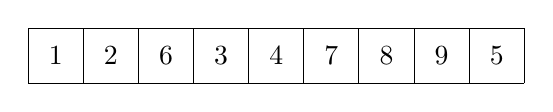
\begin{tikzpicture}[scale=0.7]
\draw (0,0) grid (9,1);

\node at (0.5,0.5) {$1$};
\node at (1.5,0.5) {$2$};
\node at (2.5,0.5) {$6$};
\node at (3.5,0.5) {$3$};
\node at (4.5,0.5) {$4$};
\node at (5.5,0.5) {$7$};
\node at (6.5,0.5) {$8$};
\node at (7.5,0.5) {$9$};
\node at (8.5,0.5) {$5$};
% 
% \footnotesize
% \node at (0.5,1.4) {$1$};
% \node at (1.5,1.4) {$2$};
% \node at (2.5,1.4) {$3$};
% \node at (3.5,1.4) {$4$};
% \node at (4.5,1.4) {$5$};
% \node at (5.5,1.4) {$6$};
% \node at (6.5,1.4) {$7$};
% \node at (7.5,1.4) {$8$};
% \node at (8.5,1.4) {$9$};
\end{tikzpicture}
\end{center}


\subsubsection{Consultes de subarbre}

Cada subarbre d'un arbre es correspon a un subvector del vector
recorregut d'arbre, on el primer element del subvector conté el
node arrel del subarbre. Per exemple, el subvector següent conté els
nodes del subarbre arrelat al node $4$:
\begin{center}
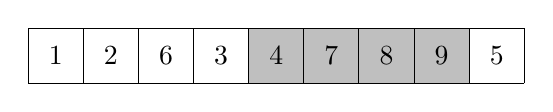
\begin{tikzpicture}[scale=0.7]
\fill[color=lightgray] (4,0) rectangle (8,1);
\draw (0,0) grid (9,1);

\node at (0.5,0.5) {$1$};
\node at (1.5,0.5) {$2$};
\node at (2.5,0.5) {$6$};
\node at (3.5,0.5) {$3$};
\node at (4.5,0.5) {$4$};
\node at (5.5,0.5) {$7$};
\node at (6.5,0.5) {$8$};
\node at (7.5,0.5) {$9$};
\node at (8.5,0.5) {$5$};
% 
% \footnotesize
% \node at (0.5,1.4) {$1$};
% \node at (1.5,1.4) {$2$};
% \node at (2.5,1.4) {$3$};
% \node at (3.5,1.4) {$4$};
% \node at (4.5,1.4) {$5$};
% \node at (5.5,1.4) {$6$};
% \node at (6.5,1.4) {$7$};
% \node at (7.5,1.4) {$8$};
% \node at (8.5,1.4) {$9$};
\end{tikzpicture}
\end{center}
Amb aquest coneixement podem processar eficientment les consultes
relacionades amb subarbres d'un arbre. Per exemple, considereu un
problema on assignem un valor a cada node i la nostra feina
és donar suport a les consultes següents:
\begin{itemize}
\item actualitzar el valor d'un node,
\item calcular la suma de valors del subarbre arrelat a un node.
\end{itemize}


Considereu l'arbre següent on els números blaus són els valors dels
nodes. Per exemple, la suma del subarbre arrelat al node $4$ és
$3+4+3+1=11$.


\begin{center}
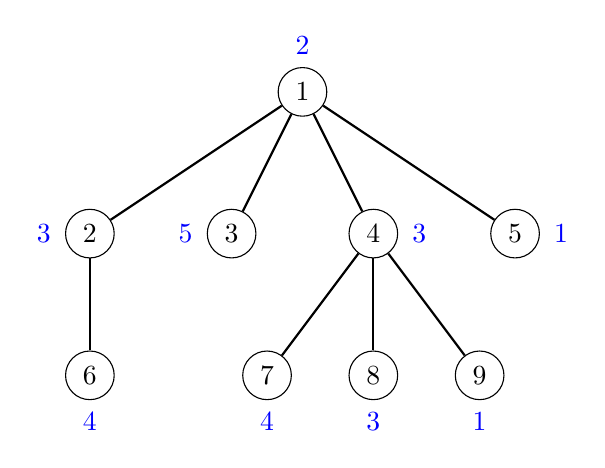
\begin{tikzpicture}[scale=0.9]
\node[draw, circle] (1) at (0,3) {$1$};
\node[draw, circle] (2) at (-3,1) {$2$};
\node[draw, circle] (3) at (-1,1) {$3$};
\node[draw, circle] (4) at (1,1) {$4$};
\node[draw, circle] (5) at (3,1) {$5$};
\node[draw, circle] (6) at (-3,-1) {$6$};
\node[draw, circle] (7) at (-0.5,-1) {$7$};
\node[draw, circle] (8) at (1,-1) {$8$};
\node[draw, circle] (9) at (2.5,-1) {$9$};

\path[draw,thick,-] (1) -- (2);
\path[draw,thick,-] (1) -- (3);
\path[draw,thick,-] (1) -- (4);
\path[draw,thick,-] (1) -- (5);
\path[draw,thick,-] (2) -- (6);
\path[draw,thick,-] (4) -- (7);
\path[draw,thick,-] (4) -- (8);
\path[draw,thick,-] (4) -- (9);

\node[color=blue] at (0,3+0.65) {2};
\node[color=blue] at (-3-0.65,1) {3};
\node[color=blue] at (-1-0.65,1) {5};
\node[color=blue] at (1+0.65,1) {3};
\node[color=blue] at (3+0.65,1) {1};
\node[color=blue] at (-3,-1-0.65) {4};
\node[color=blue] at (-0.5,-1-0.65) {4};
\node[color=blue] at (1,-1-0.65) {3};
\node[color=blue] at (2.5,-1-0.65) {1};
\end{tikzpicture}
\end{center}


La idea és construir un vector recorregut d'arbre que contingui
tres valors per cada node: l'identificador del node, la mida del
subarbre i el valor del node. Per exemple, el vector associat a
l'arbre anterior és:


\begin{center}
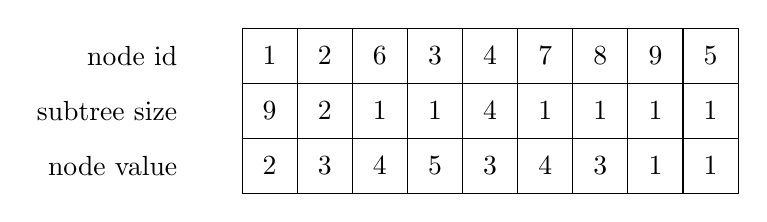
\begin{tikzpicture}[scale=0.7]
\draw (0,1) grid (9,-2);

\node[left] at (-1,0.5) {node id};
\node[left] at (-1,-0.5) {subtree size};
\node[left] at (-1,-1.5) {node value};

\node at (0.5,0.5) {$1$};
\node at (1.5,0.5) {$2$};
\node at (2.5,0.5) {$6$};
\node at (3.5,0.5) {$3$};
\node at (4.5,0.5) {$4$};
\node at (5.5,0.5) {$7$};
\node at (6.5,0.5) {$8$};
\node at (7.5,0.5) {$9$};
\node at (8.5,0.5) {$5$};

\node at (0.5,-0.5) {$9$};
\node at (1.5,-0.5) {$2$};
\node at (2.5,-0.5) {$1$};
\node at (3.5,-0.5) {$1$};
\node at (4.5,-0.5) {$4$};
\node at (5.5,-0.5) {$1$};
\node at (6.5,-0.5) {$1$};
\node at (7.5,-0.5) {$1$};
\node at (8.5,-0.5) {$1$};

\node at (0.5,-1.5) {$2$};
\node at (1.5,-1.5) {$3$};
\node at (2.5,-1.5) {$4$};
\node at (3.5,-1.5) {$5$};
\node at (4.5,-1.5) {$3$};
\node at (5.5,-1.5) {$4$};
\node at (6.5,-1.5) {$3$};
\node at (7.5,-1.5) {$1$};
\node at (8.5,-1.5) {$1$};
% 
% \footnotesize
% \node at (0.5,1.4) {$1$};
% \node at (1.5,1.4) {$2$};
% \node at (2.5,1.4) {$3$};
% \node at (3.5,1.4) {$4$};
% \node at (4.5,1.4) {$5$};
% \node at (5.5,1.4) {$6$};
% \node at (6.5,1.4) {$7$};
% \node at (7.5,1.4) {$8$};
% \node at (8.5,1.4) {$9$};
\end{tikzpicture}
\end{center}


Amb aquesta vector, podem calcular la suma de valors de qualsevol
subarbre esbrinant primer la mida del subarbre i després els valors
dels nodes corresponents. Per exemple, els valors del subarbre arrelat
al node $4$ es poden trobar de la manera següent:


\begin{center}
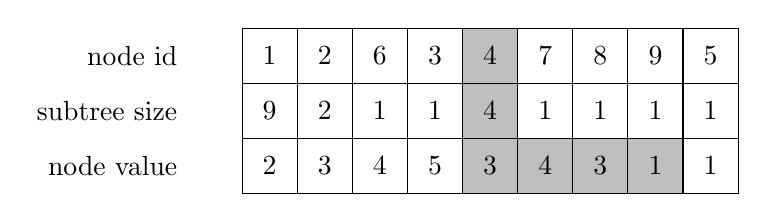
\begin{tikzpicture}[scale=0.7]
\fill[color=lightgray] (4,1) rectangle (5,0);
\fill[color=lightgray] (4,0) rectangle (5,-1);
\fill[color=lightgray] (4,-1) rectangle (8,-2);
\draw (0,1) grid (9,-2);

\node[left] at (-1,0.5) {node id};
\node[left] at (-1,-0.5) {subtree size};
\node[left] at (-1,-1.5) {node value};

\node at (0.5,0.5) {$1$};
\node at (1.5,0.5) {$2$};
\node at (2.5,0.5) {$6$};
\node at (3.5,0.5) {$3$};
\node at (4.5,0.5) {$4$};
\node at (5.5,0.5) {$7$};
\node at (6.5,0.5) {$8$};
\node at (7.5,0.5) {$9$};
\node at (8.5,0.5) {$5$};

\node at (0.5,-0.5) {$9$};
\node at (1.5,-0.5) {$2$};
\node at (2.5,-0.5) {$1$};
\node at (3.5,-0.5) {$1$};
\node at (4.5,-0.5) {$4$};
\node at (5.5,-0.5) {$1$};
\node at (6.5,-0.5) {$1$};
\node at (7.5,-0.5) {$1$};
\node at (8.5,-0.5) {$1$};

\node at (0.5,-1.5) {$2$};
\node at (1.5,-1.5) {$3$};
\node at (2.5,-1.5) {$4$};
\node at (3.5,-1.5) {$5$};
\node at (4.5,-1.5) {$3$};
\node at (5.5,-1.5) {$4$};
\node at (6.5,-1.5) {$3$};
\node at (7.5,-1.5) {$1$};
\node at (8.5,-1.5) {$1$};
% 
% \footnotesize
% \node at (0.5,1.4) {$1$};
% \node at (1.5,1.4) {$2$};
% \node at (2.5,1.4) {$3$};
% \node at (3.5,1.4) {$4$};
% \node at (4.5,1.4) {$5$};
% \node at (5.5,1.4) {$6$};
% \node at (6.5,1.4) {$7$};
% \node at (7.5,1.4) {$8$};
% \node at (8.5,1.4) {$9$};
\end{tikzpicture}
\end{center}


Per respondre les consultes de manera eficient, n'hi ha prou amb
emmagatzemar els valors dels nodes en un arbre binari indexat o
segmentat. Després d'això, podem actualitzar un valor i calcular la
suma de valors en temps $O(\log n)$.

\subsubsection{Consultes de camí}

Amb un vector recorregut d'arbre també podem calcular eficientment les
sumes de valors dels camins del node arrel a qualsevol altre node de
l'arbre. Considereu el problema on la nostra tasca és donar suport
a les consultes següents:
\begin{itemize}
\item canviar el valor d'un node,
\item calcular la suma de valors en el cami de l'arrel a un node.
\end{itemize}


Per exemple, en l'arbre següent, la suma de valors del node arrel al
node 7 és $4+5+5=14$:


\begin{center}
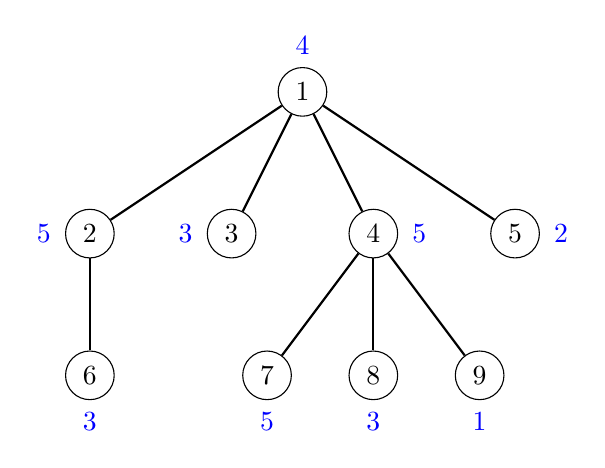
\begin{tikzpicture}[scale=0.9]
\node[draw, circle] (1) at (0,3) {$1$};
\node[draw, circle] (2) at (-3,1) {$2$};
\node[draw, circle] (3) at (-1,1) {$3$};
\node[draw, circle] (4) at (1,1) {$4$};
\node[draw, circle] (5) at (3,1) {$5$};
\node[draw, circle] (6) at (-3,-1) {$6$};
\node[draw, circle] (7) at (-0.5,-1) {$7$};
\node[draw, circle] (8) at (1,-1) {$8$};
\node[draw, circle] (9) at (2.5,-1) {$9$};

\path[draw,thick,-] (1) -- (2);
\path[draw,thick,-] (1) -- (3);
\path[draw,thick,-] (1) -- (4);
\path[draw,thick,-] (1) -- (5);
\path[draw,thick,-] (2) -- (6);
\path[draw,thick,-] (4) -- (7);
\path[draw,thick,-] (4) -- (8);
\path[draw,thick,-] (4) -- (9);

\node[color=blue] at (0,3+0.65) {4};
\node[color=blue] at (-3-0.65,1) {5};
\node[color=blue] at (-1-0.65,1) {3};
\node[color=blue] at (1+0.65,1) {5};
\node[color=blue] at (3+0.65,1) {2};
\node[color=blue] at (-3,-1-0.65) {3};
\node[color=blue] at (-0.5,-1-0.65) {5};
\node[color=blue] at (1,-1-0.65) {3};
\node[color=blue] at (2.5,-1-0.65) {1};
\end{tikzpicture}
\end{center}


Podem resoldre aquest problema com abans, però ara guardem en el
nostre vector de tuples les sumes dels camins corresponents. Per exemple, el vector
següent es correspon amb l'arbre anterior:

\begin{center}
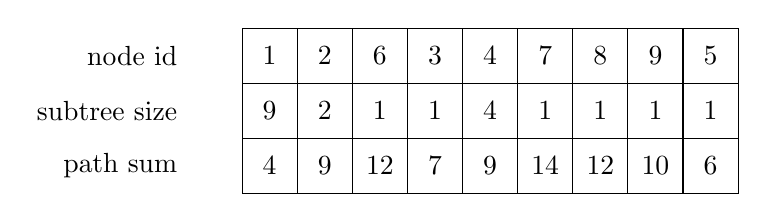
\begin{tikzpicture}[scale=0.7]
\draw (0,1) grid (9,-2);

\node[left] at (-1,0.5) {node id};
\node[left] at (-1,-0.5) {subtree size};
\node[left] at (-1,-1.5) {path sum};

\node at (0.5,0.5) {$1$};
\node at (1.5,0.5) {$2$};
\node at (2.5,0.5) {$6$};
\node at (3.5,0.5) {$3$};
\node at (4.5,0.5) {$4$};
\node at (5.5,0.5) {$7$};
\node at (6.5,0.5) {$8$};
\node at (7.5,0.5) {$9$};
\node at (8.5,0.5) {$5$};

\node at (0.5,-0.5) {$9$};
\node at (1.5,-0.5) {$2$};
\node at (2.5,-0.5) {$1$};
\node at (3.5,-0.5) {$1$};
\node at (4.5,-0.5) {$4$};
\node at (5.5,-0.5) {$1$};
\node at (6.5,-0.5) {$1$};
\node at (7.5,-0.5) {$1$};
\node at (8.5,-0.5) {$1$};

\node at (0.5,-1.5) {$4$};
\node at (1.5,-1.5) {$9$};
\node at (2.5,-1.5) {$12$};
\node at (3.5,-1.5) {$7$};
\node at (4.5,-1.5) {$9$};
\node at (5.5,-1.5) {$14$};
\node at (6.5,-1.5) {$12$};
\node at (7.5,-1.5) {$10$};
\node at (8.5,-1.5) {$6$};
\end{tikzpicture}
\end{center}


Quan el valor d'un node augmenta en $x$, les sumes dels camins de tots
els nodes del seu subarbre augmenten en $x$. Per exemple, si el valor
del node 4 augmenta en 1, el vector canvia de la següent manera:


\begin{center}
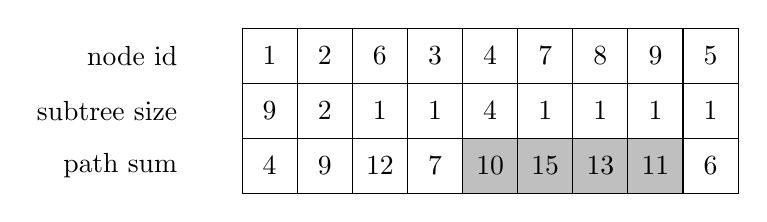
\begin{tikzpicture}[scale=0.7]
\fill[color=lightgray] (4,-1) rectangle (8,-2);
\draw (0,1) grid (9,-2);

\node[left] at (-1,0.5) {node id};
\node[left] at (-1,-0.5) {subtree size};
\node[left] at (-1,-1.5) {path sum};

\node at (0.5,0.5) {$1$};
\node at (1.5,0.5) {$2$};
\node at (2.5,0.5) {$6$};
\node at (3.5,0.5) {$3$};
\node at (4.5,0.5) {$4$};
\node at (5.5,0.5) {$7$};
\node at (6.5,0.5) {$8$};
\node at (7.5,0.5) {$9$};
\node at (8.5,0.5) {$5$};

\node at (0.5,-0.5) {$9$};
\node at (1.5,-0.5) {$2$};
\node at (2.5,-0.5) {$1$};
\node at (3.5,-0.5) {$1$};
\node at (4.5,-0.5) {$4$};
\node at (5.5,-0.5) {$1$};
\node at (6.5,-0.5) {$1$};
\node at (7.5,-0.5) {$1$};
\node at (8.5,-0.5) {$1$};

\node at (0.5,-1.5) {$4$};
\node at (1.5,-1.5) {$9$};
\node at (2.5,-1.5) {$12$};
\node at (3.5,-1.5) {$7$};
\node at (4.5,-1.5) {$10$};
\node at (5.5,-1.5) {$15$};
\node at (6.5,-1.5) {$13$};
\node at (7.5,-1.5) {$11$};
\node at (8.5,-1.5) {$6$};
\end{tikzpicture}
\end{center}


Així, podem implementar les dues operacions si som capaços d'augmentar
tots els valors d'un interval i recuperar un sol valor. Això es pot
fer en temps $O(\log n)$ fent servir arbre binari indexat o segmentat
(vegeu el capítol~\ref{actualitzacio-d-intervals}).

\section{Avantpassat comú més baix}

\index{avantpassat comú més baix}

La \key{avantpassat comú més baix} de dos nodes d'un arbre arrelat és
el node més baix que conté ambdós nodes en el seu subarbre. Un
problema típic és respondre eficientment consultes d'aquest tipus.

Per exemple, a l'arbre següent, l'avantpassat comú més baix dels nodes
5 i 8 és el node 2:
\begin{center}
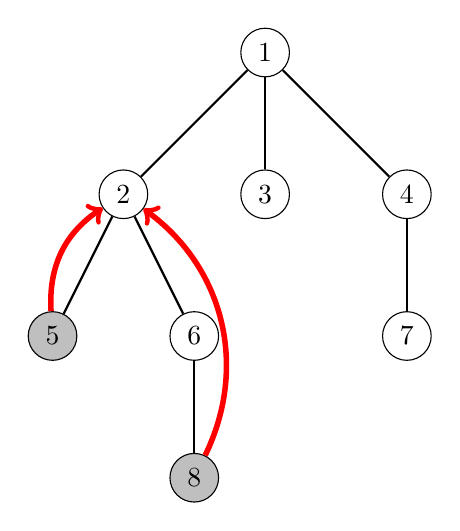
\begin{tikzpicture}[scale=0.9]
\node[draw, circle] (1) at (0,3) {$1$};
\node[draw, circle] (2) at (2,1) {$4$};
\node[draw, circle] (3) at (-2,1) {$2$};
\node[draw, circle] (4) at (0,1) {$3$};
\node[draw, circle] (5) at (2,-1) {$7$};
\node[draw, circle, fill=lightgray] (6) at (-3,-1) {$5$};
\node[draw, circle] (7) at (-1,-1) {$6$};
\node[draw, circle, fill=lightgray] (8) at (-1,-3) {$8$};
\path[draw,thick,-] (1) -- (2);
\path[draw,thick,-] (1) -- (3);
\path[draw,thick,-] (1) -- (4);
\path[draw,thick,-] (2) -- (5);
\path[draw,thick,-] (3) -- (6);
\path[draw,thick,-] (3) -- (7);
\path[draw,thick,-] (7) -- (8);

\path[draw=red,thick,->,line width=2pt] (6) edge [bend left] (3);
\path[draw=red,thick,->,line width=2pt] (8) edge [bend right=40] (3);
\end{tikzpicture}
\end{center}


A continuació, mostrem dues tècniques eficients per trobar
l'avantpassat comú més baix de dos nodes.

\subsubsection{Mètode 1}

Una manera de resoldre el problema és fer servir que podem trobar de
manera eficient el $k$-èssim avantpassat de qualsevol node de
l'arbre. Amb això, podem dividir el problema de trobar l'avantpassat
comú més baix en dues parts.

Fem servir dos punters que apunten inicialment als dos nodes. Primer,
movem un dels punters cap amunt fins que que ambdós punters estiguin a
la mateixa alçada.

En l'escenari d'exemple, movem el segon punter un nivell cap
amunt. Ara apunta al node 6, que es troba al mateix nivell que el node
5:


\begin{center}
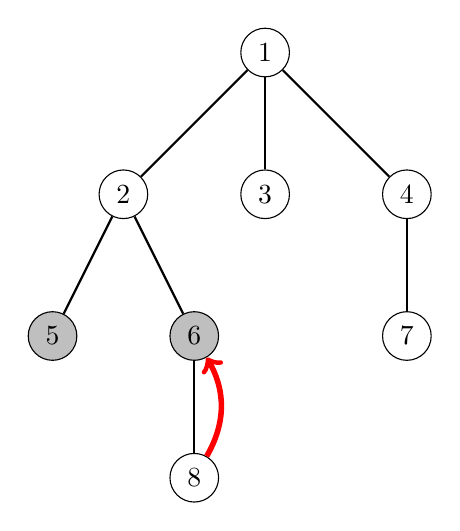
\begin{tikzpicture}[scale=0.9]
\node[draw, circle] (1) at (0,3) {$1$};
\node[draw, circle] (2) at (2,1) {$4$};
\node[draw, circle] (3) at (-2,1) {$2$};
\node[draw, circle] (4) at (0,1) {$3$};
\node[draw, circle] (5) at (2,-1) {$7$};
\node[draw, circle,fill=lightgray] (6) at (-3,-1) {$5$};
\node[draw, circle,fill=lightgray] (7) at (-1,-1) {$6$};
\node[draw, circle] (8) at (-1,-3) {$8$};
\path[draw,thick,-] (1) -- (2);
\path[draw,thick,-] (1) -- (3);
\path[draw,thick,-] (1) -- (4);
\path[draw,thick,-] (2) -- (5);
\path[draw,thick,-] (3) -- (6);
\path[draw,thick,-] (3) -- (7);
\path[draw,thick,-] (7) -- (8);

\path[draw=red,thick,->,line width=2pt] (8) edge [bend right] (7);
\end{tikzpicture}
\end{center}


Després d'això, trobem el mínim nombre de passos necessaris cap a
amunt per a que els dos punters apuntin al mateix node. Aquest node és
l'avantpassat comú més baix.

En l'escenari d'exemple, n'hi ha prou amb moure els dos punters un pas
cap amunt fins al node 2, que és l'avantpassat comú més baix:


\begin{center}
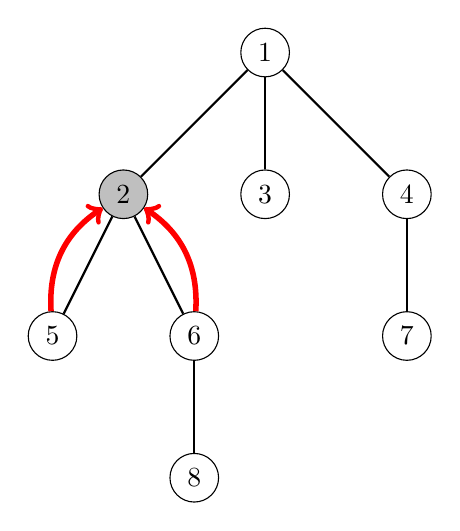
\begin{tikzpicture}[scale=0.9]
\node[draw, circle] (1) at (0,3) {$1$};
\node[draw, circle] (2) at (2,1) {$4$};
\node[draw, circle,fill=lightgray] (3) at (-2,1) {$2$};
\node[draw, circle] (4) at (0,1) {$3$};
\node[draw, circle] (5) at (2,-1) {$7$};
\node[draw, circle] (6) at (-3,-1) {$5$};
\node[draw, circle] (7) at (-1,-1) {$6$};
\node[draw, circle] (8) at (-1,-3) {$8$};
\path[draw,thick,-] (1) -- (2);
\path[draw,thick,-] (1) -- (3);
\path[draw,thick,-] (1) -- (4);
\path[draw,thick,-] (2) -- (5);
\path[draw,thick,-] (3) -- (6);
\path[draw,thick,-] (3) -- (7);
\path[draw,thick,-] (7) -- (8);

\path[draw=red,thick,->,line width=2pt] (6) edge [bend left] (3);
\path[draw=red,thick,->,line width=2pt] (7) edge [bend right] (3);
\end{tikzpicture}
\end{center}


Les dos parts de l'algorisme es poden realitzar en temps $O(\log n)$
amb informació precalculada, de manera que podem trobar l'avantpassat
comú més baix de dos nodes qualsevols en temps $O(\log n)$.

\subsubsection{Mètode 2}

Una altra manera de resoldre el problema es basa en un vector
recorregut d'arbre\footnote{Aquest algorisme d'avantpassat comú més
baix es va presentar a \cite{ben00}. Aquesta tècnica de vegades
s'anomena \index{tècnica de recorregut d'Euler} \key{tècnica de
  recorregut d'Euler} \cite{tar84}.}. Una vegada més, la idea és
d'avançar pels nodes amb una cerca en profunditat:


\begin{center}
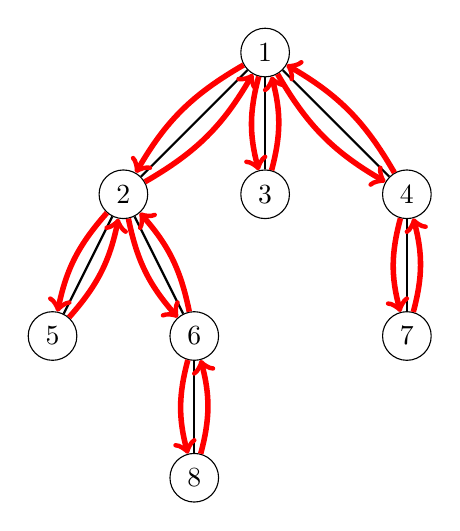
\begin{tikzpicture}[scale=0.9]
\node[draw, circle] (1) at (0,3) {$1$};
\node[draw, circle] (2) at (2,1) {$4$};
\node[draw, circle] (3) at (-2,1) {$2$};
\node[draw, circle] (4) at (0,1) {$3$};
\node[draw, circle] (5) at (2,-1) {$7$};
\node[draw, circle] (6) at (-3,-1) {$5$};
\node[draw, circle] (7) at (-1,-1) {$6$};
\node[draw, circle] (8) at (-1,-3) {$8$};
\path[draw,thick,-] (1) -- (2);
\path[draw,thick,-] (1) -- (3);
\path[draw,thick,-] (1) -- (4);
\path[draw,thick,-] (2) -- (5);
\path[draw,thick,-] (3) -- (6);
\path[draw,thick,-] (3) -- (7);
\path[draw,thick,-] (7) -- (8);

\path[draw=red,thick,->,line width=2pt] (1) edge [bend right=15] (3);
\path[draw=red,thick,->,line width=2pt] (3) edge [bend right=15] (6);
\path[draw=red,thick,->,line width=2pt] (6) edge [bend right=15] (3);
\path[draw=red,thick,->,line width=2pt] (3) edge [bend right=15] (7);
\path[draw=red,thick,->,line width=2pt] (7) edge [bend right=15] (8);
\path[draw=red,thick,->,line width=2pt] (8) edge [bend right=15] (7);
\path[draw=red,thick,->,line width=2pt] (7) edge [bend right=15] (3);
\path[draw=red,thick,->,line width=2pt] (3) edge [bend right=15] (1);
\path[draw=red,thick,->,line width=2pt] (1) edge [bend right=15] (4);
\path[draw=red,thick,->,line width=2pt] (4) edge [bend right=15] (1);
\path[draw=red,thick,->,line width=2pt] (1) edge [bend right=15] (2);
\path[draw=red,thick,->,line width=2pt] (2) edge [bend right=15] (5);
\path[draw=red,thick,->,line width=2pt] (5) edge [bend right=15] (2);
\path[draw=red,thick,->,line width=2pt] (2) edge [bend right=15] (1);
\end{tikzpicture}
\end{center}


Ara, però, fem servir un vector recorregut d'arbre diferent de
l'anterior: afegim cada node al vector \emph{sempre} que la cerca en
profunditat passa pel node, i no només la primera vegada que el
veiem. Per tant, un node amb $k$ fills apareix $k+1$ vegades al
vector, i el vecor conté $2n-1$ elements.

Emmagatzemem dos valors al vector: l'identificador del node i la
profunditat del node a l'arbre. El vector següent es correspon amb
l'arbre anterior:


\begin{center}
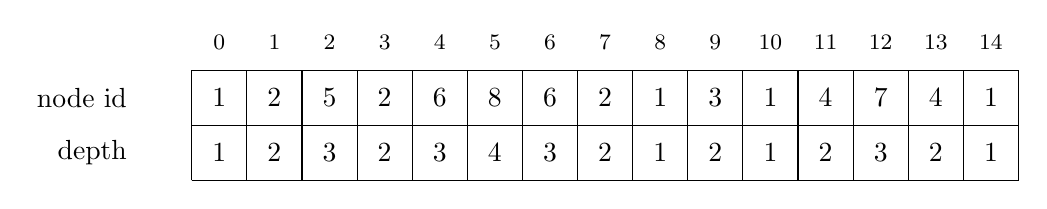
\begin{tikzpicture}[scale=0.7]

\node[left] at (-1,1.5) {node id};
\node[left] at (-1,0.5) {depth};

\draw (0,1) grid (15,2);
\node at (0.5,1.5) {$1$};
\node at (1.5,1.5) {$2$};
\node at (2.5,1.5) {$5$};
\node at (3.5,1.5) {$2$};
\node at (4.5,1.5) {$6$};
\node at (5.5,1.5) {$8$};
\node at (6.5,1.5) {$6$};
\node at (7.5,1.5) {$2$};
\node at (8.5,1.5) {$1$};
\node at (9.5,1.5) {$3$};
\node at (10.5,1.5) {$1$};
\node at (11.5,1.5) {$4$};
\node at (12.5,1.5) {$7$};
\node at (13.5,1.5) {$4$};
\node at (14.5,1.5) {$1$};

\draw (0,0) grid (15,1);
\node at (0.5,0.5) {$1$};
\node at (1.5,0.5) {$2$};
\node at (2.5,0.5) {$3$};
\node at (3.5,0.5) {$2$};
\node at (4.5,0.5) {$3$};
\node at (5.5,0.5) {$4$};
\node at (6.5,0.5) {$3$};
\node at (7.5,0.5) {$2$};
\node at (8.5,0.5) {$1$};
\node at (9.5,0.5) {$2$};
\node at (10.5,0.5) {$1$};
\node at (11.5,0.5) {$2$};
\node at (12.5,0.5) {$3$};
\node at (13.5,0.5) {$2$};
\node at (14.5,0.5) {$1$};

\footnotesize
\node at (0.5,2.5) {$0$};
\node at (1.5,2.5) {$1$};
\node at (2.5,2.5) {$2$};
\node at (3.5,2.5) {$3$};
\node at (4.5,2.5) {$4$};
\node at (5.5,2.5) {$5$};
\node at (6.5,2.5) {$6$};
\node at (7.5,2.5) {$7$};
\node at (8.5,2.5) {$8$};
\node at (9.5,2.5) {$9$};
\node at (10.5,2.5) {$10$};
\node at (11.5,2.5) {$11$};
\node at (12.5,2.5) {$12$};
\node at (13.5,2.5) {$13$};
\node at (14.5,2.5) {$14$};
\end{tikzpicture}
\end{center}


Ara podem trobar l'avantpassat comú més baix dels nodes $a$ i $b$
trobant el node amb profunditat \emph{mínima} entre els nodes $a$ i
$b$ del vector. Per exemple, l'avantpassat comú més baix dels nodes
$5$ i $8$ es pot trobar de la següent manera:


\begin{center}
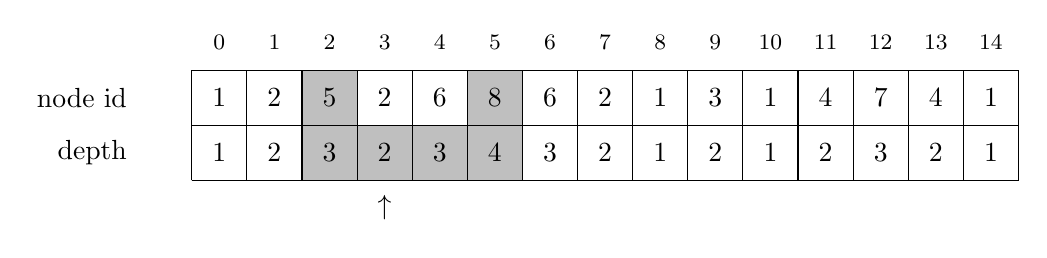
\begin{tikzpicture}[scale=0.7]

\node[left] at (-1,1.5) {node id};
\node[left] at (-1,0.5) {depth};

\fill[color=lightgray] (2,1) rectangle (3,2);
\fill[color=lightgray] (5,1) rectangle (6,2);
\fill[color=lightgray] (2,0) rectangle (6,1);

\node at (3.5,-0.5) {$\uparrow$};

\draw (0,1) grid (15,2);
\node at (0.5,1.5) {$1$};
\node at (1.5,1.5) {$2$};
\node at (2.5,1.5) {$5$};
\node at (3.5,1.5) {$2$};
\node at (4.5,1.5) {$6$};
\node at (5.5,1.5) {$8$};
\node at (6.5,1.5) {$6$};
\node at (7.5,1.5) {$2$};
\node at (8.5,1.5) {$1$};
\node at (9.5,1.5) {$3$};
\node at (10.5,1.5) {$1$};
\node at (11.5,1.5) {$4$};
\node at (12.5,1.5) {$7$};
\node at (13.5,1.5) {$4$};
\node at (14.5,1.5) {$1$};


\draw (0,0) grid (15,1);
\node at (0.5,0.5) {$1$};
\node at (1.5,0.5) {$2$};
\node at (2.5,0.5) {$3$};
\node at (3.5,0.5) {$2$};
\node at (4.5,0.5) {$3$};
\node at (5.5,0.5) {$4$};
\node at (6.5,0.5) {$3$};
\node at (7.5,0.5) {$2$};
\node at (8.5,0.5) {$1$};
\node at (9.5,0.5) {$2$};
\node at (10.5,0.5) {$1$};
\node at (11.5,0.5) {$2$};
\node at (12.5,0.5) {$3$};
\node at (13.5,0.5) {$2$};
\node at (14.5,0.5) {$1$};

\footnotesize
\node at (0.5,2.5) {$0$};
\node at (1.5,2.5) {$1$};
\node at (2.5,2.5) {$2$};
\node at (3.5,2.5) {$3$};
\node at (4.5,2.5) {$4$};
\node at (5.5,2.5) {$5$};
\node at (6.5,2.5) {$6$};
\node at (7.5,2.5) {$7$};
\node at (8.5,2.5) {$8$};
\node at (9.5,2.5) {$9$};
\node at (10.5,2.5) {$10$};
\node at (11.5,2.5) {$11$};
\node at (12.5,2.5) {$12$};
\node at (13.5,2.5) {$13$};
\node at (14.5,2.5) {$14$};
\end{tikzpicture}
\end{center}


El node 5 es troba a la posició 2, el node 8 es troba a la posició 5 i
el node de profunditat mínima entre les posicions $2 \ldots 5$ és el
node 2 a la posició 3, i té profunditat 2. Així, l'avantpassat comú
més baix dels nodes 5 i 8 és el node 2.

Per tant, per trobar l'avantpassat comú més baix de dos nodes n'hi ha
prou amb processar una consulta d'interval mínim. Com que el vector és
estàtic, podem processar consultes com aquesta en temps $O(1)$ després
del preprocessament de temps $O(n \log n)$.

\subsubsection{Distàncies dels nodes}

La distància entre els nodes $a$ i $b$ és igual a la longitud del camí
de $a$ a $b$. Resulta que el problema de calcular la distància entre
dos nodes es redueix a trobar el seu avantpassat comú més baix.

Primer, arrelem l'arbre de manera arbitrària. Després d'això, la
distància dels nodes $a$ i $b$ es pot calcular mitjançant la fórmula
\[\texttt{depth}(a)+\texttt{depth}(b)-2 \cdot \texttt{depth}(c),\]
on $c$ és l'avantpassat comú més baix de $a$ i $b$ i
$\texttt{depth}(s)$ indica la profunditat del node $s$. Per exemple,
considereu la distància entre els nodes 5 i 8:
\begin{center}
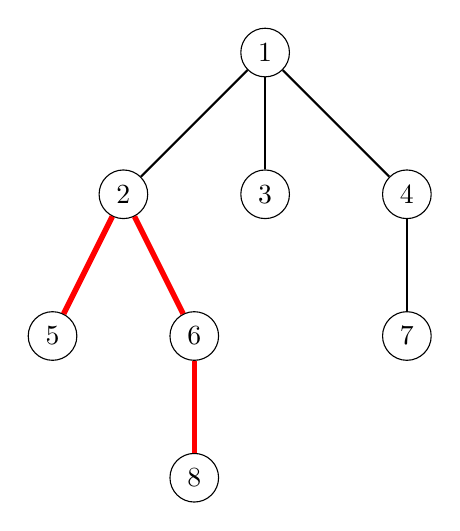
\begin{tikzpicture}[scale=0.9]
\node[draw, circle] (1) at (0,3) {$1$};
\node[draw, circle] (2) at (2,1) {$4$};
\node[draw, circle] (3) at (-2,1) {$2$};
\node[draw, circle] (4) at (0,1) {$3$};
\node[draw, circle] (5) at (2,-1) {$7$};
\node[draw, circle] (6) at (-3,-1) {$5$};
\node[draw, circle] (7) at (-1,-1) {$6$};
\node[draw, circle] (8) at (-1,-3) {$8$};
\path[draw,thick,-] (1) -- (2);
\path[draw,thick,-] (1) -- (3);
\path[draw,thick,-] (1) -- (4);
\path[draw,thick,-] (2) -- (5);
\path[draw,thick,-] (3) -- (6);
\path[draw,thick,-] (3) -- (7);
\path[draw,thick,-] (7) -- (8);

\path[draw=red,thick,-,line width=2pt] (8) -- node[font=\small] {} (7);
\path[draw=red,thick,-,line width=2pt] (7) -- node[font=\small] {} (3);
\path[draw=red,thick,-,line width=2pt] (6) -- node[font=\small] {} (3);
\end{tikzpicture}
\end{center}


L'avantpassat comú més baix dels nodes 5 i 8 és el node 2. Les
profunditats dels nodes són $\texttt{depth}(5)=3$,
$\texttt{depth}(8)=4$ i $\texttt{depth}(2)=2$, de manera que la
distància entre els nodes 5 i 8 és $3+4-2\cdot2=3$.

\section{Algorismes \emph{offline}}

Fins ara, hem tractat els algorismes \emph{online} de consultes
d'arbres. Aquests algorismes són capaços de processar les consultes
una rera l'altra de manera que cada consulta es respon abans de rebre
la següent.

Tanmateix, en molts problemes, no és necessari fer-ho així. En aquesta
secció ens centrem en els algorismes \emph{offline}. Aquests
algorismes reben un conjunt de consultes que es permés respondre en
qualsevol ordre. Sovint és més fàcil dissenyar un algorisme \emph{offline} que no
pas un algorisme online.

\subsubsection{Fusionar estructures de dades}

Un mètode per construir algorismes \emph{offline} és fer un recorregut
de l'arbre en profunditat i mantenir estructures de dades als
nodes. Per cada node $s$, creem una estructura de dades
$\texttt{d}[s]$ que es basa en les estructures de dades dels fills de
$s$. Aleshores, fem servir aquesta estructura de dades per processar
totes les consultes relacionades amb $s$.

Com a exemple, considereu el problema següent: donat un arbre on cada
node té algun valor, processa consultes de la forma ''troba el nombre
de nodes amb valor $x$ al subarbre del node $s$''. Per exemple, a
l'arbre següent, el subarbre arrelat al node $4$ conté dos nodes el valor
dels quals és 3.


\begin{center}
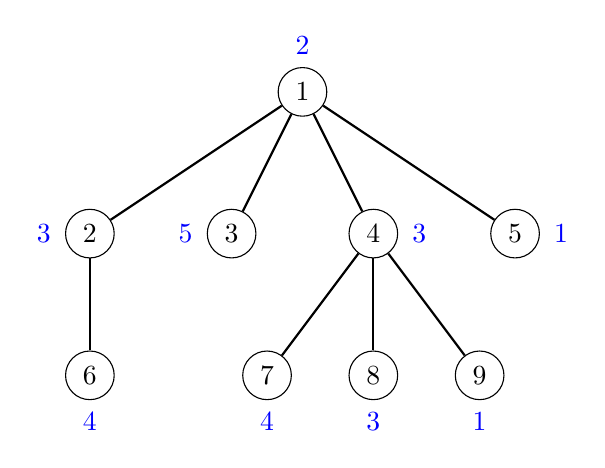
\begin{tikzpicture}[scale=0.9]
\node[draw, circle] (1) at (0,3) {$1$};
\node[draw, circle] (2) at (-3,1) {$2$};
\node[draw, circle] (3) at (-1,1) {$3$};
\node[draw, circle] (4) at (1,1) {$4$};
\node[draw, circle] (5) at (3,1) {$5$};
\node[draw, circle] (6) at (-3,-1) {$6$};
\node[draw, circle] (7) at (-0.5,-1) {$7$};
\node[draw, circle] (8) at (1,-1) {$8$};
\node[draw, circle] (9) at (2.5,-1) {$9$};

\path[draw,thick,-] (1) -- (2);
\path[draw,thick,-] (1) -- (3);
\path[draw,thick,-] (1) -- (4);
\path[draw,thick,-] (1) -- (5);
\path[draw,thick,-] (2) -- (6);
\path[draw,thick,-] (4) -- (7);
\path[draw,thick,-] (4) -- (8);
\path[draw,thick,-] (4) -- (9);

\node[color=blue] at (0,3+0.65) {2};
\node[color=blue] at (-3-0.65,1) {3};
\node[color=blue] at (-1-0.65,1) {5};
\node[color=blue] at (1+0.65,1) {3};
\node[color=blue] at (3+0.65,1) {1};
\node[color=blue] at (-3,-1-0.65) {4};
\node[color=blue] at (-0.5,-1-0.65) {4};
\node[color=blue] at (1,-1-0.65) {3};
\node[color=blue] at (2.5,-1-0.65) {1};
\end{tikzpicture}
\end{center}


En aquest problema, podem fem servir mapes per respondre les
consultes. Per exemple, els mapes per al node 4 i els seus fills són
els següents:


\begin{center}
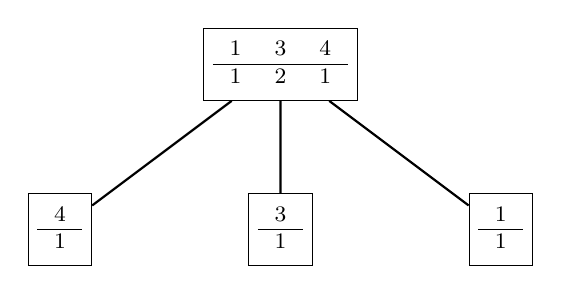
\begin{tikzpicture}[scale=0.7]

\node[draw, rectangle] (a) at (4,5.5)
{
\footnotesize
\begin{tabular}{rrr}
4 \\
\hline
1 \\
\end{tabular}};

\node[draw, rectangle] (b) at (8,5.5)
{
\footnotesize
\begin{tabular}{rrr}
3 \\
\hline
1 \\
\end{tabular}};


\node[draw, rectangle] (c) at (12,5.5)
{
\footnotesize
\begin{tabular}{rr}
1 \\
\hline
1 \\
\end{tabular}};

\node[draw, rectangle] (d) at (8,8.5)
{
\footnotesize
\begin{tabular}{rrr}
1 & 3 & 4 \\
\hline
1 & 2 & 1 \\
\end{tabular}};
\path[draw,thick,-] (a) -- (d);
\path[draw,thick,-] (b) -- (d);
\path[draw,thick,-] (c) -- (d);
\end{tikzpicture}
\end{center}


Si creem una estructura de dades com aquesta per a cada node, podem
processar fàcilment totes les consultes relacionades amb un node donat
just després de crear l'estructura de dades pel node en
questió. Per exemple, el mapa anterior ens
indica que el subarbre arrelat al node 4 conté dos nodes el valor dels
quals és 3.

Tanmateix, seria massa lent crear totes les estructures de dades des
de zero. En canvi, per cada node $s$, creem una estructura de dades
inicial $\texttt{d}[s]$ que només conté el valor de $s$. Després
d'això, recorrem els fills $u$ de $s$ i \emph{fusionem}
$\texttt{d}[s]$ i totes les estructures de dades
$\texttt{d}[u]$ \footnote{(N. del T.) I, un cop finalitzada la fusió
de $\texttt{d}[s]$, responem totes les consultes relatives al node
$s$. Això ens obliga a ordenar les consultes en post-ordre.}.

Per exemple, en l'arbre anterior, el mapa del node $4$ es crea
fusionant els mapes següents:


\begin{center}
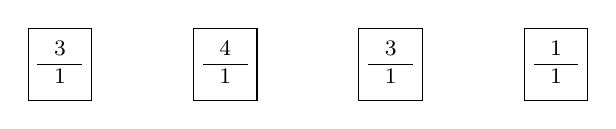
\begin{tikzpicture}[scale=0.7]

\node[draw, rectangle] (a) at (4,5.5)
{
\footnotesize
\begin{tabular}{rrr}
4 \\
\hline
1 \\
\end{tabular}};

\node[draw, rectangle] (b) at (7,5.5)
{
\footnotesize
\begin{tabular}{rrr}
3 \\
\hline
1 \\
\end{tabular}};

\node[draw, rectangle] (c) at (10,5.5)
{
\footnotesize
\begin{tabular}{rr}
1 \\
\hline
1 \\
\end{tabular}};

\node[draw, rectangle] (d) at (1,5.5)
{
\footnotesize
\begin{tabular}{rr}
3 \\
\hline
1 \\
\end{tabular}};

\end{tikzpicture}
\end{center}


El primer mapa és l'estructura de dades inicial del node 4, i els
altres tres mapes corresponen als nodes 7, 8 i 9.

La fusió al node $s$ es pot fer de la següent manera: per cada fill
$u$ de $s$ fusionem $\texttt{d}[s]$ i $\texttt{d}[u]$. Fem la fusió
copiant el contingut de $\texttt{d}[u]$ sobre $\texttt{d}[s]$, però si
la mida de $\texttt{d}[s]$ és més petita que la mida de
$\texttt{d}[u]$, intercanviem (\emph{swap}) els continguts dels mapes
abans de fer la fusió. Fent això cada valor només es copia $O(\log n)$
vegades durant el recorregut d'arbre\footnote{(N. del T.): Això no és
cert: és possible construir contra-exemples d'alçada $\sqrt{n}$ on un
mapa es copia $\sqrt{n}$ vegades. Tot i això, l'algorisme sí és
eficient, pel següent motiu. Considerem un algorisme semblant al
nostre però on en lloc de fer \emph{swap}s en funció de la mida dels
mapes $\texttt{d}[s]$ i $\texttt{d}[u]$, fem sempre un únic
\emph{swap} entre $\texttt{d}[s]$ i $\texttt{d}[u_{max}]$, on
$u_{max}$ és un fill de $s$ amb subarbre de mida màxima, i els mapes
$\texttt{d}[u]$ de la resta de fills es copien a sobre d'aquest. (Això
es coneix com ``\emph{small to large}''). Aquest algorisme calcula els
mateixos mapes que l'algorisme original, però fa igual o més feina en
les fusions, perquè no fa servir el criteri òptim per estalviar-se
còpies. Amb aquest canvi es compleix que tots els mapes es copien
$O(\log n)$ vegades, ja que només copiem un mapa $\texttt{d}[u]$ sobre
$\texttt{d}[s]$ si l'arbre arrelat a $s$ és el doble de gran que
l'arbre arrelat a $u$. Com que comencem amb $n$ mapes de mida $1$, el
cost total de l'algorisme és $O(n\log n)$. I d'aquí deduïm que
l'algorisme original també té cost total $O(n\log n)$.}, la qual cosa
garanteix que l'algorisme és eficient.

Podem intercanviar el contingut de dues estructures de dades $a$ i $b$
de manera eficient fent servir:
\begin{lstlisting}
swap(a,b);
\end{lstlisting}
El codi anterior sempre funciona en temps constant quan $a$ i $b$ són
estructures de dades de la biblioteca estàndard de C++.

\subsubsection{Avantpassats comuns més baixos}

També hi ha un algorisme \emph{offline} per processar un conjunt de
consultes d'avantpassats comuns més baixos\footnote{Aquest algorisme
va ser publicat per R. E. Tarjan el 1979 \cite{tar79}.}. L'algorisme
es basa en l'estructura \emph{union-find} (vegeu el
capítol~\ref{union-find}), i un benefici és que és més fàcil
d'implementar que els algorismes presentats anteriorment.

L'algorisme rep com a entrada un conjunt de parells de nodes i
determina, per a cada parell, l'avantpassat comú més baix dels
nodes. L'algorisme realitza una travessa de l'arbre a la profunditat i
manté una estructura \emph{union-find}, on inicialment cada node
pertany a un conjunt separat. Per a cada conjunt emmagatzemem també el
node més alt que pertany al conjunt.

Quan l'algorisme visita un node $x$, processa totes les consultes de
la forma $(x,y)$ on $y$ ja ha estat visitat amb anterioritat, i respon
que l'avantpassat comú més baix de $x$ i $y$ és el node més alt del
conjunt associat a $y$. Un cop hem acabat de processar el node $x$
l'algorisme uneix els conjunts de $x$ i el seu pare.

Per exemple, suposem que volem trobar els avantpassats comuns més
baixos dels parells de nodes $(5,8)$ i $(2,7)$ a l'arbre següent:
\begin{center}
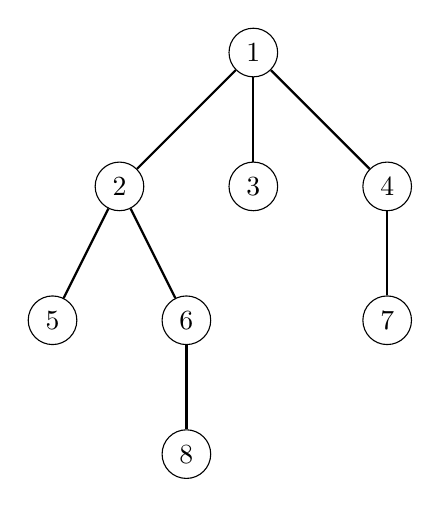
\begin{tikzpicture}[scale=0.85]
\node[draw, circle] (1) at (0,3) {$1$};
\node[draw, circle] (2) at (2,1) {$4$};
\node[draw, circle] (3) at (-2,1) {$2$};
\node[draw, circle] (4) at (0,1) {$3$};
\node[draw, circle] (5) at (2,-1) {$7$};
\node[draw, circle] (6) at (-3,-1) {$5$};
\node[draw, circle] (7) at (-1,-1) {$6$};
\node[draw, circle] (8) at (-1,-3) {$8$};
\path[draw,thick,-] (1) -- (2);
\path[draw,thick,-] (1) -- (3);
\path[draw,thick,-] (1) -- (4);
\path[draw,thick,-] (2) -- (5);
\path[draw,thick,-] (3) -- (6);
\path[draw,thick,-] (3) -- (7);
\path[draw,thick,-] (7) -- (8);
\end{tikzpicture}
\end{center}


En els arbres següents, els nodes grisos denoten nodes visitats i els
grups de nodes amb guions pertanyen al mateix conjunt. Quan
l'algorisme visita el node 8, s'adona que el node 5 ja ha estat
visitat i que el node més alt del conjunt corresponent és 2. Per tant,
l'avantpassat comú més baix dels nodes 5 i 8 és 2:
\begin{center}
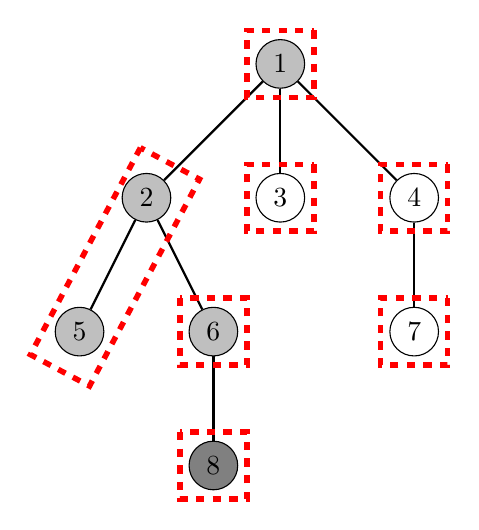
\begin{tikzpicture}[scale=0.85]
\node[draw, circle, fill=lightgray] (1) at (0,3) {$1$};
\node[draw, circle] (2) at (2,1) {$4$};
\node[draw, circle, fill=lightgray] (3) at (-2,1) {$2$};
\node[draw, circle] (4) at (0,1) {$3$};
\node[draw, circle] (5) at (2,-1) {$7$};
\node[draw, circle, fill=lightgray] (6) at (-3,-1) {$5$};
\node[draw, circle, fill=lightgray] (7) at (-1,-1) {$6$};
\node[draw, circle, fill=gray] (8) at (-1,-3) {$8$};
\path[draw,thick,-] (1) -- (2);
\path[draw,thick,-] (1) -- (3);
\path[draw,thick,-] (1) -- (4);
\path[draw,thick,-] (2) -- (5);
\path[draw,thick,-] (3) -- (6);
\path[draw,thick,-] (3) -- (7);
\path[draw,thick,-] (7) -- (8);

\draw [red,thick,dashed,line width=2pt,rotate around={-28:(-2,0)}] (-2.9,1.5) rectangle (-1.9,-2);


\draw [red,thick,dashed,line width=2pt] (-1.5,-0.5) rectangle (-0.5,-1.5);
\draw [red,thick,dashed,line width=2pt] (-1.5,-2.5) rectangle (-0.5,-3.5);

\draw [red,thick,dashed,line width=2pt] (0.5,3.5) rectangle (-0.5,2.5);
\draw [red,thick,dashed,line width=2pt] (0.5,1.5) rectangle (-0.5,0.5);
\draw [red,thick,dashed,line width=2pt] (2.5,1.5) rectangle (1.5,0.5);
\draw [red,thick,dashed,line width=2pt] (2.5,-0.5) rectangle (1.5,-1.5);
\end{tikzpicture}
\end{center}


Més tard, en visitar el node 7, l'algorisme determina que
l'avantpassat comú més baix dels nodes 2 i 7 és 1:
\begin{center}
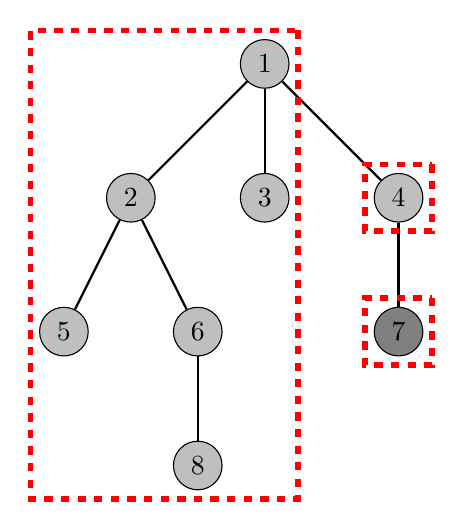
\begin{tikzpicture}[scale=0.85]
\node[draw, circle, fill=lightgray] (1) at (0,3) {$1$};
\node[draw, circle, fill=lightgray] (2) at (2,1) {$4$};
\node[draw, circle, fill=lightgray] (3) at (-2,1) {$2$};
\node[draw, circle, fill=lightgray] (4) at (0,1) {$3$};
\node[draw, circle, fill=gray] (5) at (2,-1) {$7$};
\node[draw, circle, fill=lightgray] (6) at (-3,-1) {$5$};
\node[draw, circle, fill=lightgray] (7) at (-1,-1) {$6$};
\node[draw, circle, fill=lightgray] (8) at (-1,-3) {$8$};
\path[draw,thick,-] (1) -- (2);
\path[draw,thick,-] (1) -- (3);
\path[draw,thick,-] (1) -- (4);
\path[draw,thick,-] (2) -- (5);
\path[draw,thick,-] (3) -- (6);
\path[draw,thick,-] (3) -- (7);
\path[draw,thick,-] (7) -- (8);

\draw [red,thick,dashed,line width=2pt] (0.5,3.5) rectangle (-3.5,-3.5);
\draw [red,thick,dashed,line width=2pt] (2.5,1.5) rectangle (1.5,0.5);
\draw [red,thick,dashed,line width=2pt] (2.5,-0.5) rectangle (1.5,-1.5);

\end{tikzpicture}
\end{center}
